% Preamble
\documentclass[11pt]{article}
\usepackage{graphicx}
\usepackage[margin=1in]{geometry}

\usepackage{makeidx}  % allows for indexgeneration
\usepackage{ifpdf}
\usepackage{url}


\title{Center Column Equalities in Elementary Cellular Automata}
\date{November 2024}
\author{Daniel McKinley}

% Document
\begin{document}

    \maketitle


    \section{Introduction}
% Document
    Elementary cellular automata (ECA) are extensions of logic gate truth tables done linearly iteratively
    in parallel \cite{Wolfram}. Any given center column of an input neighborhood surrounded by
    zeros has multiple alternate input neighborhoods of larger sizes producing the same center
    column with a predictable phase offset. The brute force method of attempting all possible
    neighborhoods for equivalent center columns is trimmed to ??? via Wolfram code extensions
    beyond row 1. Output for this algorithm is tested via brute force and several kinds of behavior
    for various classes of rules are explored. The algorithm is applied to Wolfram's prime number
    cellular automata \cite{Wolfram} and all Java source code is available at \cite{mygit}\\
    \section{Main Algorithm}
    \begin{center}
    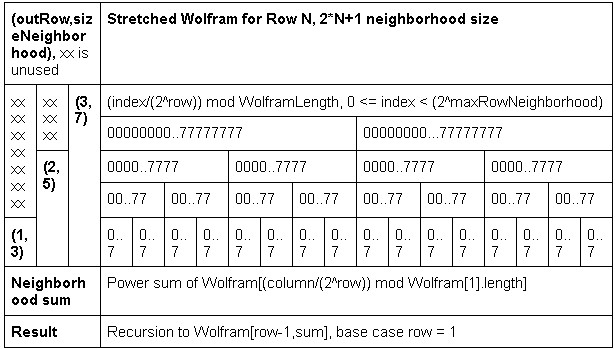
\includegraphics{RuleStretch}\\
    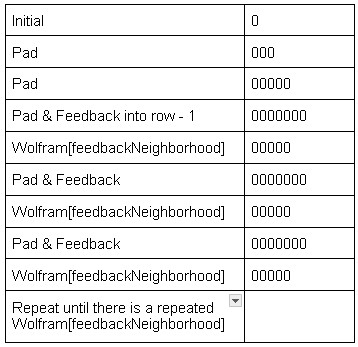
\includegraphics{StretchFeedback}
        \end{center}
	\section{Properties}

    \subsection{Row offset}
    \subsection{Distribution within all possible neighborhoods}
    \subsubsection{30, Class 4}
    \subsubsection{XOR additive}
        \subsection{ECA O(n)}
    \subsection{Applied to Prime Automata}
    \cite{Wolfram}

    \bibliographystyle{plain}
    \bibliography{CenterColumnBib}


\end{document}